\documentclass[11pt,a4paper]{report}

\usepackage{fontspec}
\setmainfont{Noto Serif CJK SC}
\setsansfont{Noto Sans CJK SC}

\XeTeXlinebreaklocale "zh"
\XeTeXlinebreakskip = 0pt plus 1pt
\sloppy
\emergencystretch=3em

\usepackage[margin=1.0in]{geometry}
\usepackage{graphicx}
\usepackage{xcolor}
\usepackage{xurl}
\usepackage{hyperref}
\usepackage{booktabs}
\usepackage{tcolorbox}
\usepackage{enumitem}
\usepackage{amsmath,amssymb}
\usepackage{titlesec}
\usepackage{fancyhdr}

\definecolor{hiveNavy}{RGB}{15,23,42}
\definecolor{hiveCyan}{RGB}{2,132,199}
\definecolor{hiveAmber}{RGB}{217,119,6}
\definecolor{hiveEmerald}{RGB}{5,150,105}
\definecolor{hiveCoral}{RGB}{220,38,38}
\definecolor{hivePurple}{RGB}{124,58,237}
\definecolor{hiveGrayBg}{RGB}{248,250,252}

\hypersetup{
    colorlinks=true,
    linkcolor=hiveCyan,
    citecolor=hiveEmerald,
    urlcolor=hiveCyan,
    pdftitle={Project HiveMind: Citizen AI & The Decentralized GPU Cooperative},
    pdfauthor={Xavier Callens and Project HiveMind Collective}
}

\tcbset{
    boxrule=1pt,
    arc=4pt,
    colback=hiveGrayBg,
    colframe=hiveCyan!80!black,
    fonttitle=\bfseries\color{white},
    colbacktitle=hiveNavy
}

\pagestyle{fancy}
\fancyhf{}
\lhead{\footnotesize \textbf{Project HiveMind} --- Citizen AI Multilingual Guide}
\rhead{\footnotesize EN $\cdot$ FR $\cdot$ ES $\cdot$ 中文 $\cdot$ DE}
\cfoot{\thepage}

\begin{document}

% ============================================================================
% TITLE PAGE
% ============================================================================
\begin{titlepage}
    \centering
    \vspace*{1.5cm}
    
    {\Huge \bfseries \color{hiveNavy} Project HiveMind}\\[0.4cm]
    {\LARGE \bfseries \color{hiveCyan} Citizen AI \& The Decentralized GPU Cooperative}\\[0.8cm]
    {\large \bfseries The Science, Technology, Market Equilibrium \& Real Results Explained for Everyone}\\[1.5cm]
    
    \begin{tcolorbox}[colback=hiveCyan!10, colframe=hiveCyan, width=0.92\textwidth]
        \centering \small \bfseries
        Available in Five Languages / Disponible en Cinq Langues / Disponible en Cinco Idiomas / 五种语言完整版 / Verfügbar in Fünf Sprachen:\\[0.3em]
        \color{hiveNavy} English $\cdot$ Français $\cdot$ Español $\cdot$ 简体中文 $\cdot$ Deutsch
    \end{tcolorbox}
    
    \vspace{1.2cm}
    
    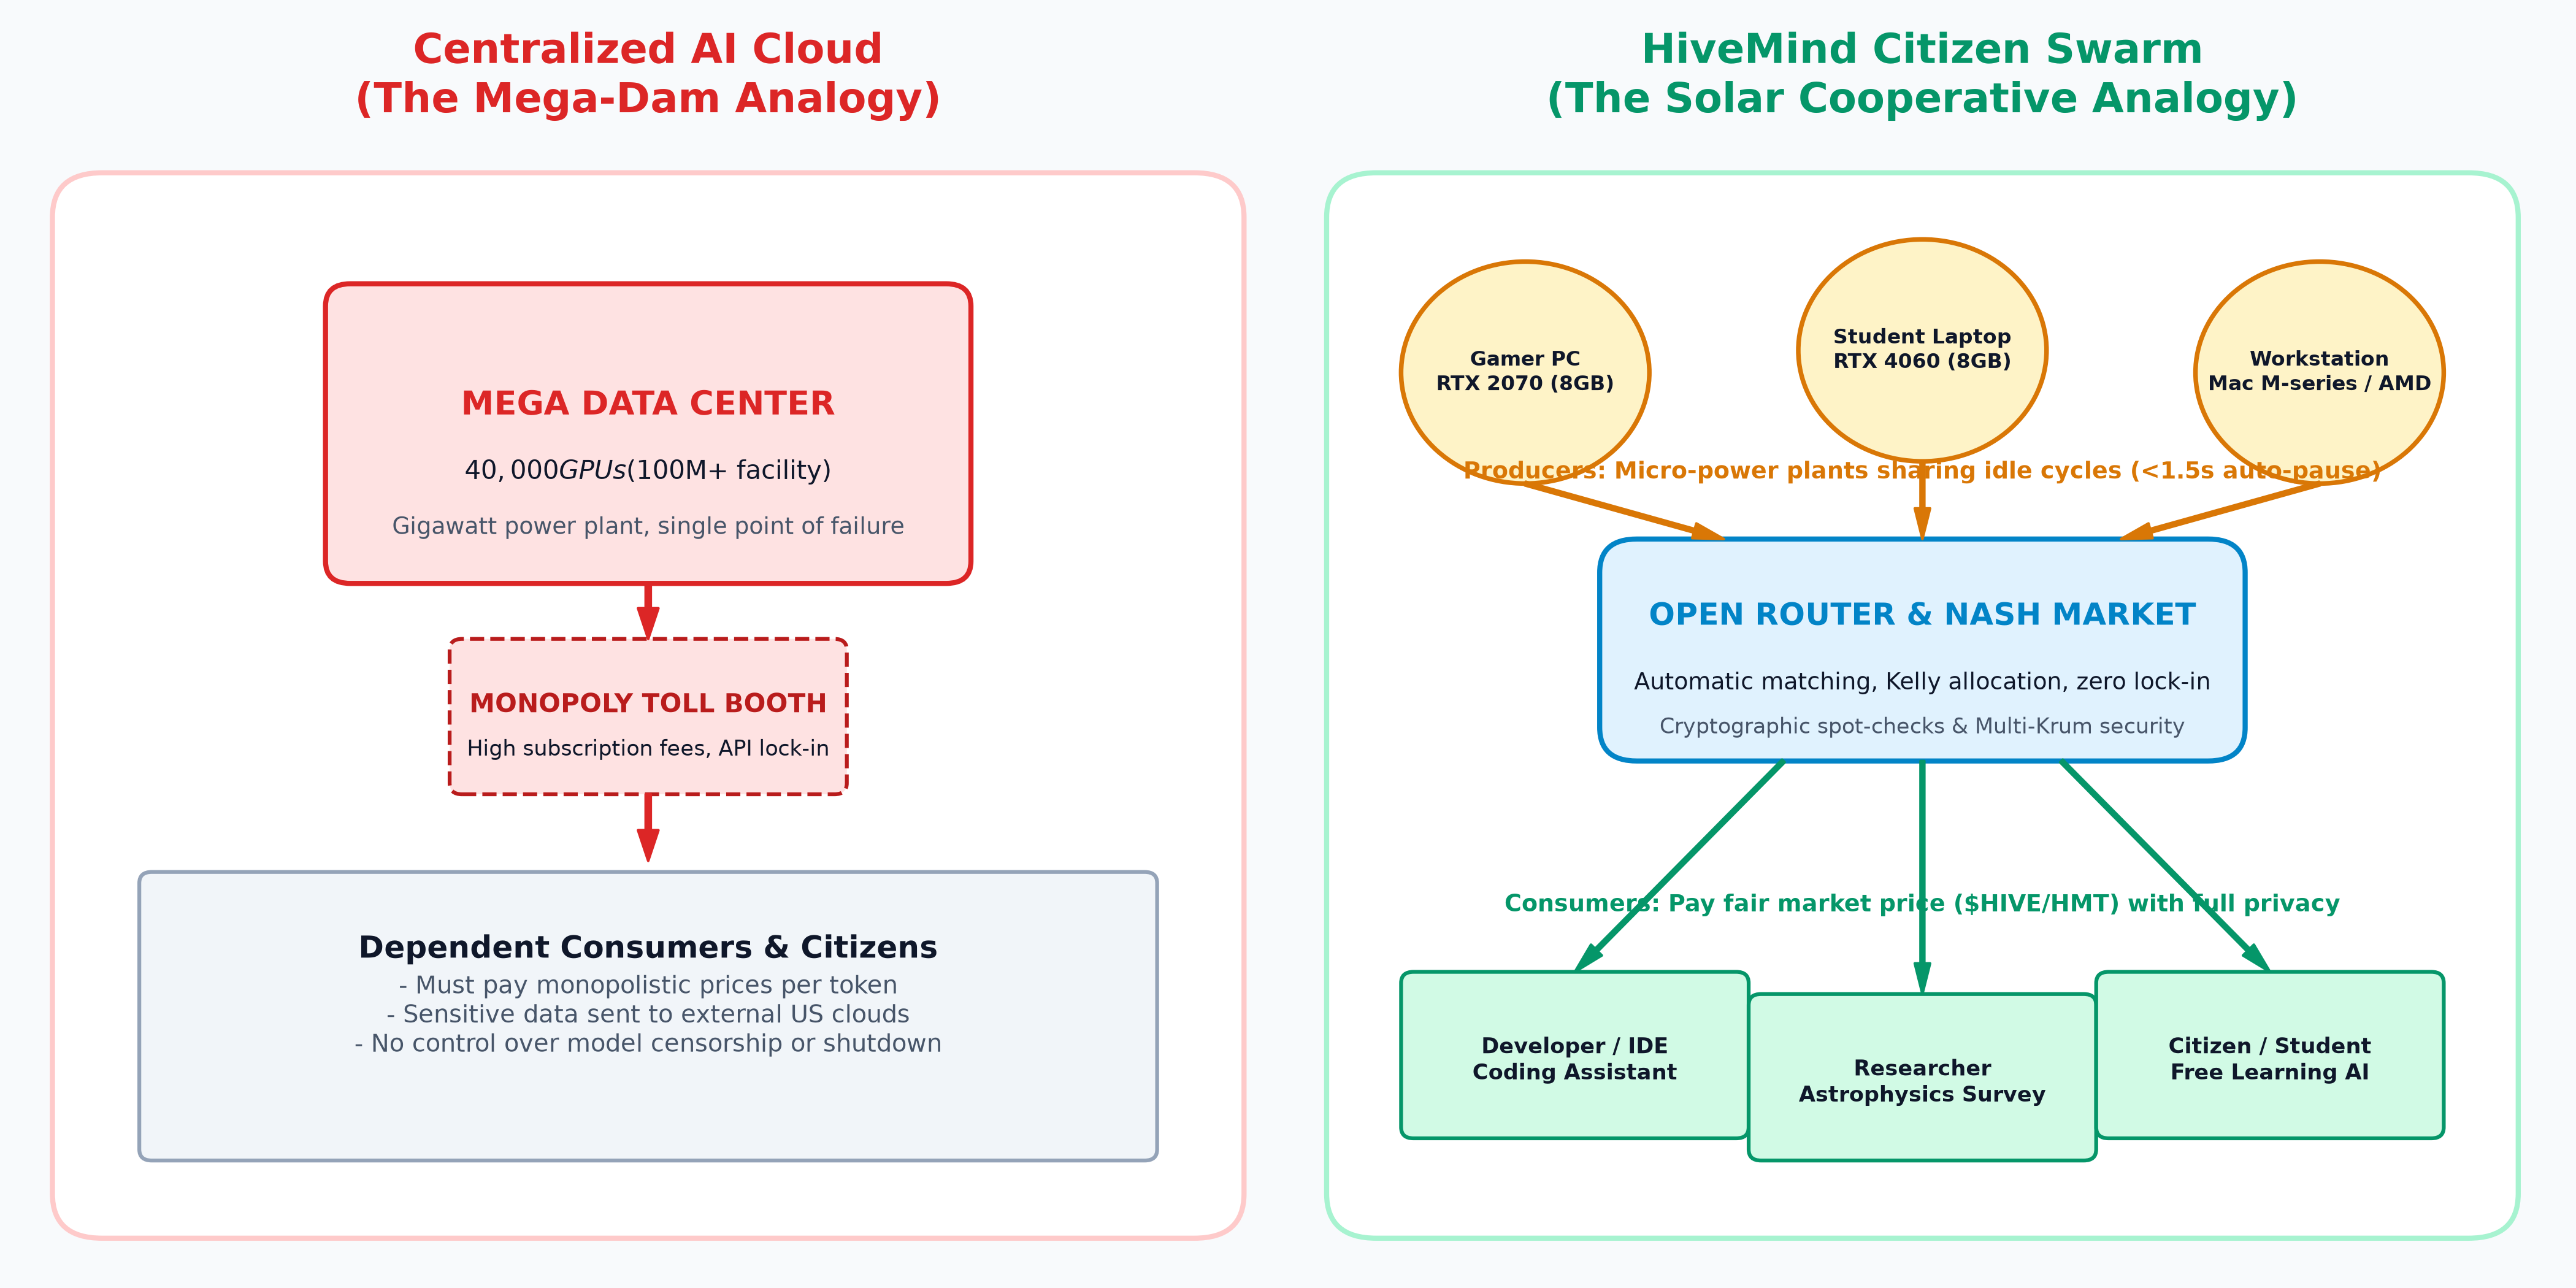
\includegraphics[width=0.85\textwidth]{figures/fig1_everyday_analogy.png}
    
    \vfill
    
    {\normalsize \textbf{Author:} Xavier Callens \& The Project HiveMind Open-Source Swarm Collective}\\[0.2cm]
    {\small Open-Source Citizen Science \& Decentralized Intelligence}\\[0.2cm]
    {\footnotesize Live Gateway: \url{https://hivemind-openrouter-1003063861791.us-central1.run.app/}}\\[0.2cm]
    {\footnotesize Zenodo DOI: \texttt{10.5281/zenodo.22829767} $\cdot$ October 2026}
\end{titlepage}

\tableofcontents
\newpage

% ============================================================================
% CHAPTER 1: ENGLISH EDITION
% ============================================================================
\chapter{English Edition: Citizen AI for Everyone}
\label{chap:en}

\section{The Big Picture: Monopoly Dams vs. The Rooftop Solar Cooperative}

Today, the world of Artificial Intelligence is dominated by a handful of tech titans. Training and running modern Large Language Models (LLMs) currently requires massive data centers housing tens of thousands of specialized, industrial-grade graphics cards (such as the NVIDIA H100, which costs over \$40,000 each). 

\paragraph{The Everyday Analogy: The Giant Hydroelectric Dam.}
Think of today's centralized AI like a massive, privately owned hydroelectric dam controlling the only river in a region. Everyone needs electricity (AI intelligence), but to get it, you must pay whatever toll the dam owner demands. If they decide to double prices, censor your usage, shut down your favorite application, or inspect your private information, you have no choice. The entire region is vulnerable to a single point of failure.

\paragraph{The HiveMind Alternative: The Rooftop Solar Cooperative.}
Project HiveMind approaches AI the way modern clean energy approaches the electrical grid: through \textbf{distributed rooftop solar panels}. 
Across the globe, gamers, students, software engineers, and small businesses already own hundreds of millions of everyday computers with consumer graphics cards (GPUs with 8~GB of memory, such as an NVIDIA GeForce RTX 2070 or RTX 4060, Apple M-series chips, or AMD Radeon cards). 

Individually, an 8~GB GPU cannot train a 100-billion-parameter AI model. But when connected together through HiveMind's mathematical protocols, millions of modest citizen GPUs form a \textbf{collective supercomputer} capable of training, fine-tuning, and serving state-of-the-art AI models without any centralized corporate bottleneck.

\begin{figure}[ht!]
    \centering
    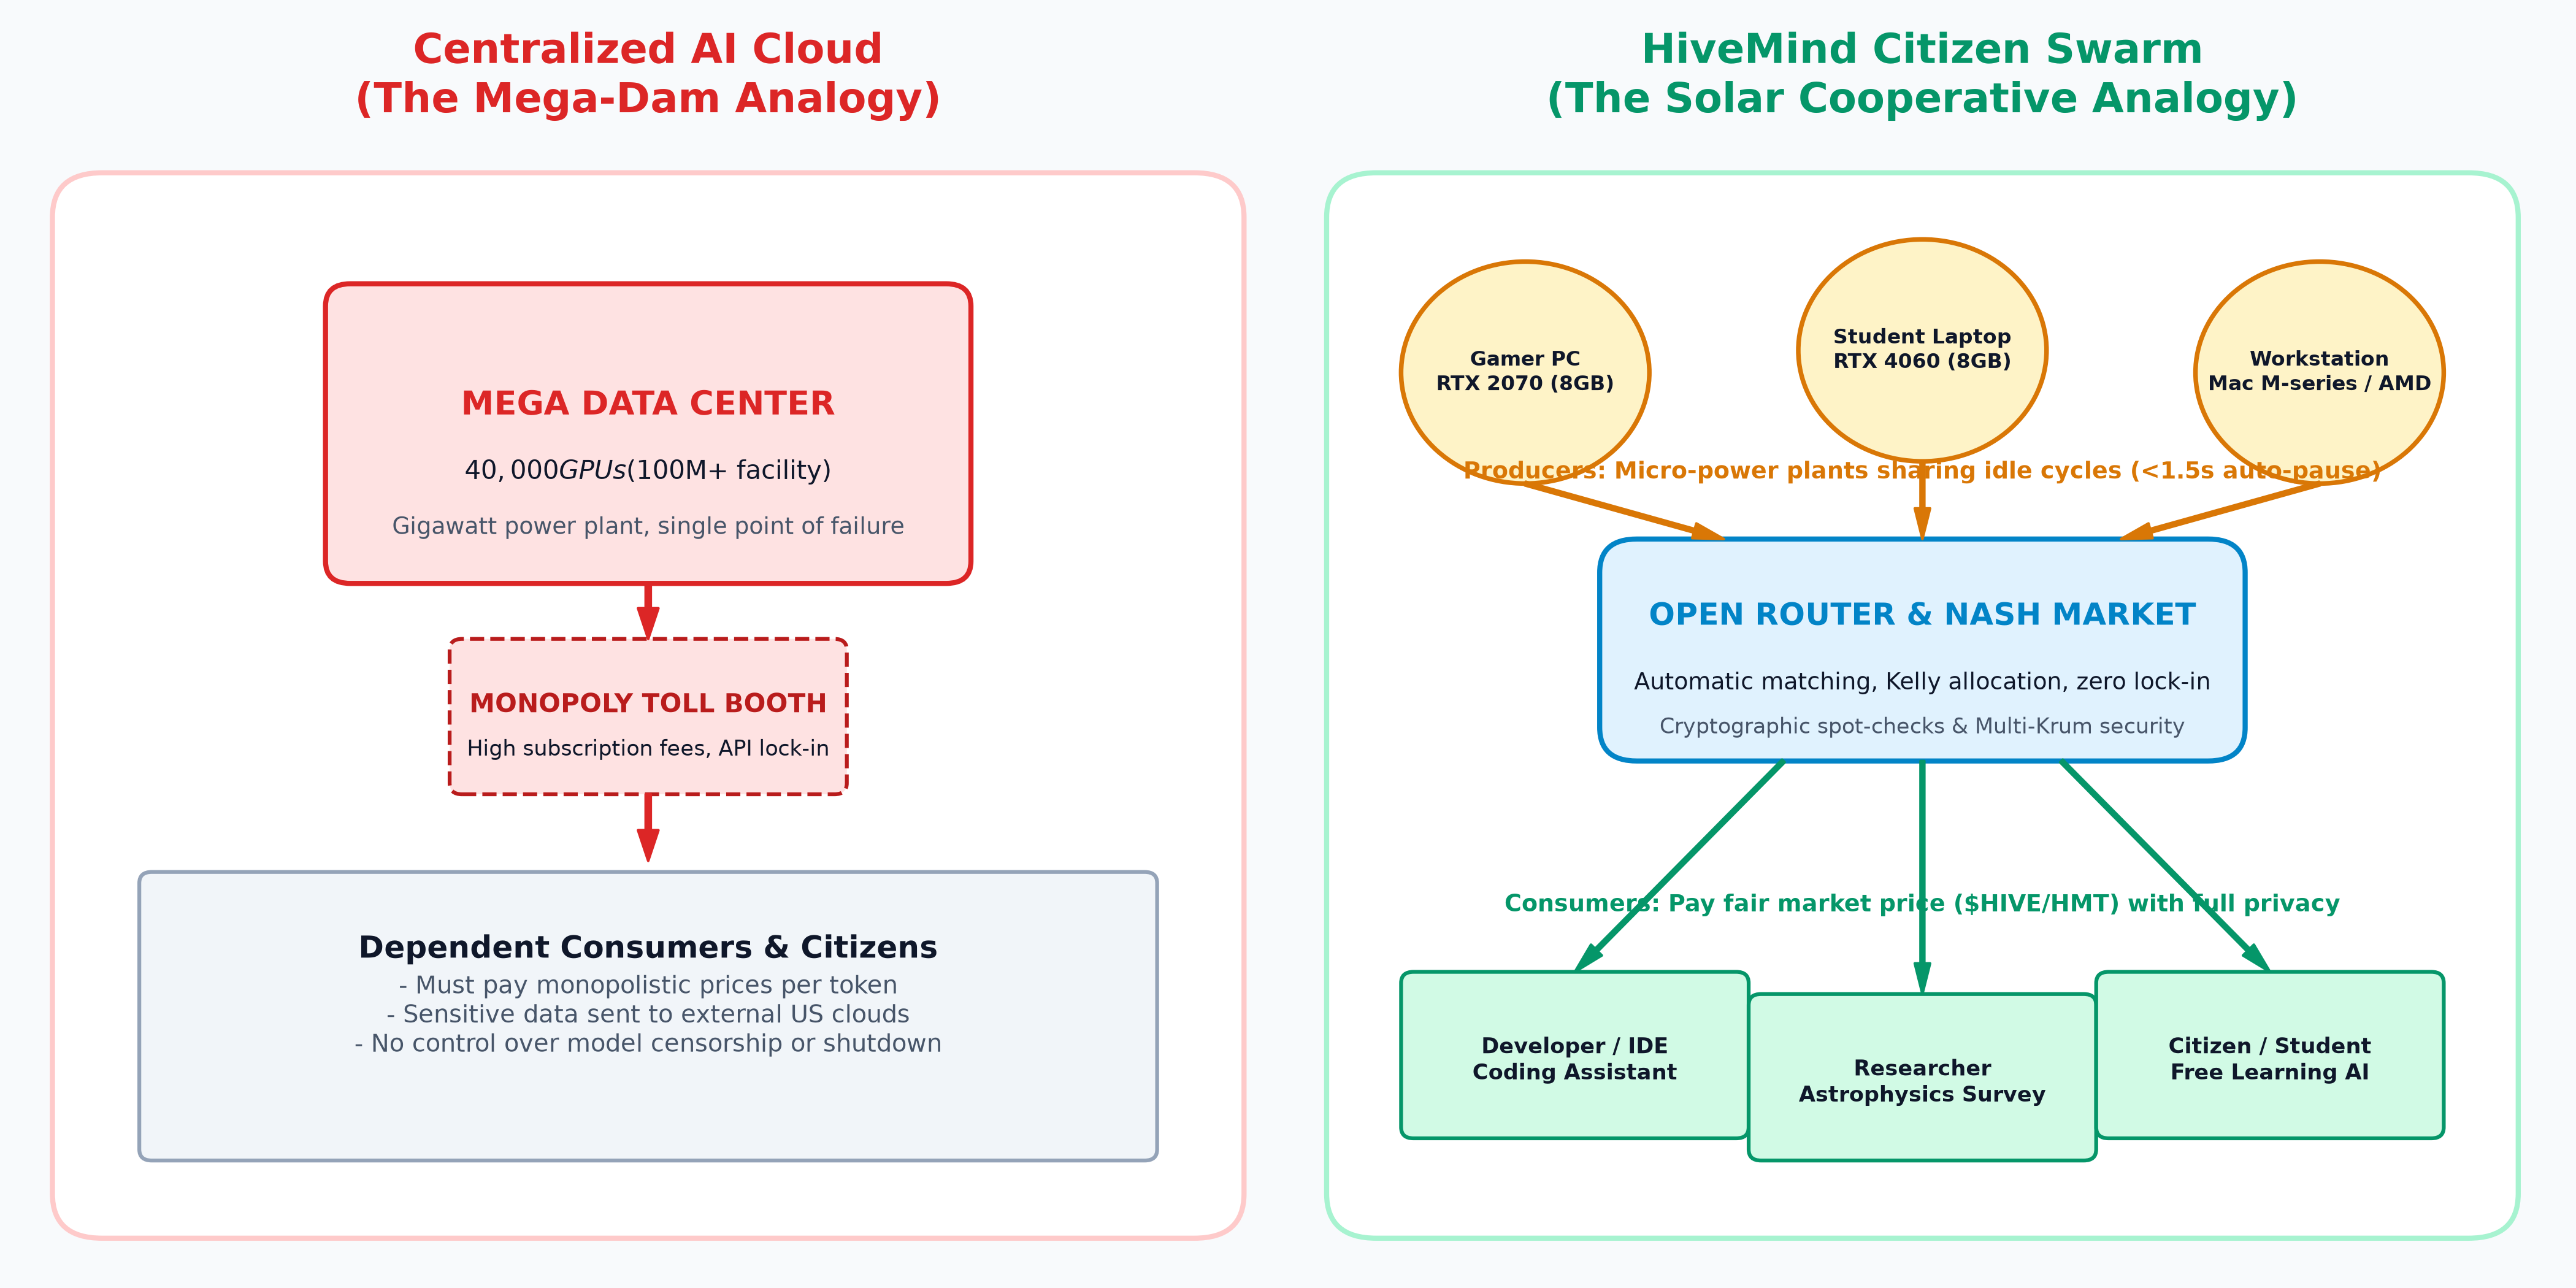
\includegraphics[width=0.92\textwidth]{figures/fig1_everyday_analogy.png}
    \caption{Everyday life analogy: Centralized big tech cloud monopoly (left) versus the HiveMind citizen solar/beehive cooperative (right).}
    \label{fig:en_analogy}
\end{figure}

\section{Breaking the Walls: How 8 GB GPUs Do Supercomputer Work}

Two physical barriers traditionally made training large AI across home internet impossible: the \textbf{VRAM Wall} (home GPUs don't have enough memory) and the \textbf{Bandwidth Wall} (home residential internet is 1,000 times slower than data center optical cables). HiveMind solves both through elegant mathematics:

\begin{itemize}[leftmargin=1.8em]
    \item \textbf{4-Bit NormalFloat (NF4) Meta-Device Streaming:} Instead of loading an entire gigantic model into memory at once, HiveMind compresses model weights to 4 bits and streams only active layers into memory as calculations happen, allowing a 96-expert Mixture-of-Experts (MoE) brain to run in less than 2~GB of VRAM!
    \item \textbf{DiLoCo Asynchronous Training with 2-Bit DCT Compression:} Instead of communicating back and forth after every microscopic calculation (which would freeze home internet), each volunteer worker computes 500 local learning steps independently. When syncing, gradient changes are compressed into 2-bit frequency representations (DCT), slashing internet bandwidth consumption by \textbf{99.9\%}.
    \item \textbf{FoMoE (Federated Mixture-of-Experts) \& Skip-Tokens:} Like a hospital where doctors specialize (cardiology, neurology, pediatrics), the AI model is divided into 128 specialist ``experts''. Each volunteer GPU only hosts 8 to 16 resident experts. When a question is processed, tokens are routed to available specialists; if an expert is on an offline machine, it ``skips'' without crashing the network.
    \item \textbf{Zero-Trust Security (Multi-Krum \& 10\% Spot-Checks):} What if a rogue node lies or submits fake calculations? HiveMind randomly spot-checks 10\% of all computing segments by replaying them bit-by-bit. If a node cheats, it receives zero credit and is filtered out by Byzantine consensus algorithms.
\end{itemize}

\section{The OpenRouter: Smart Matching of Consumers and Producers}

The \textbf{HiveMind OpenRouter} is an open gateway that works just like familiar AI APIs. Any developer can plug HiveMind into their favorite coding tools (Cursor, VSCode, Cline, Aider, OpenCode) simply by pointing the API address to the HiveMind gateway.

\begin{figure}[ht!]
    \centering
    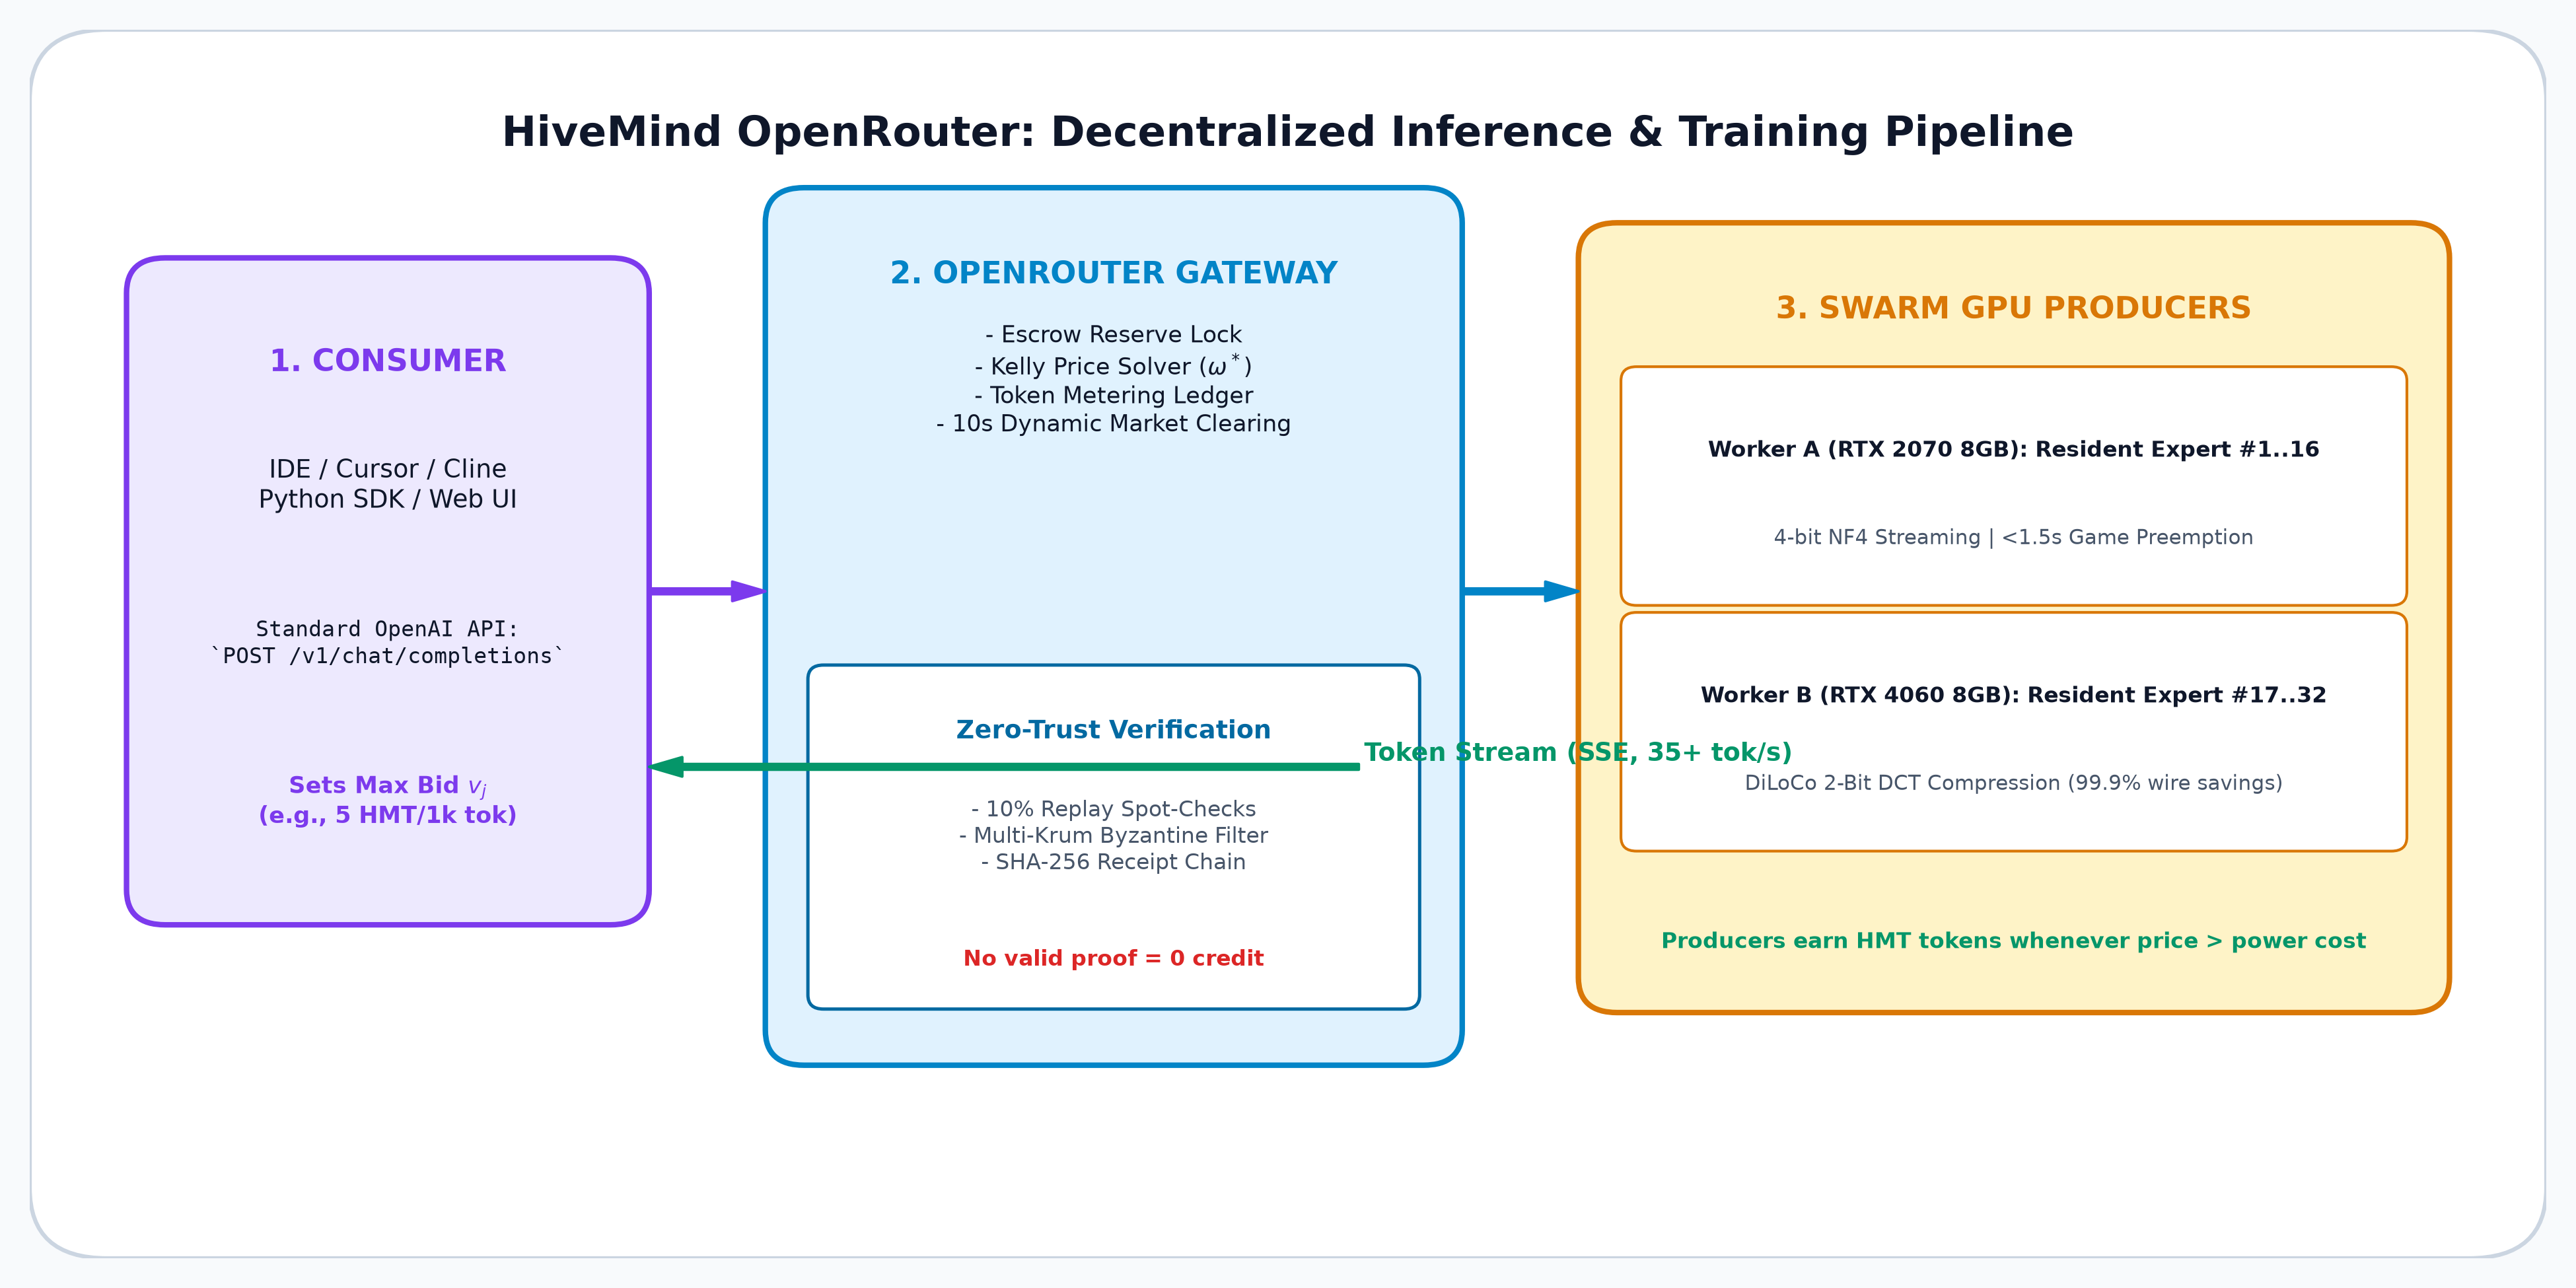
\includegraphics[width=0.95\textwidth]{figures/fig2_openrouter_architecture.png}
    \caption{The HiveMind OpenRouter pipeline: Prompts from developers and citizens are routed to decentralized volunteer GPUs with escrow protection and zero-trust verification.}
    \label{fig:en_openrouter}
\end{figure}

\begin{enumerate}[leftmargin=1.8em]
    \item \textbf{Consumers (Developers, Students, Citizens):} Send chat prompts, coding queries, or research tasks. You pay a fair market price per 1,000 tokens using compute points ($HMT$ / $\$HIVE$), protected by a temporary escrow lock.
    \item \textbf{Producers (Gamers, GPU Owners):} Run a lightweight background worker. When your GPU is idle, it processes tokens for the network and earns tokens.
    \item \textbf{Instant Streaming:} Responses stream back to your screen at 35+ tokens per second with round-trip latency under 100~ms.
\end{enumerate}

\section{The Double-Sided Nash Equilibrium: Why Everyone Wins}

How does HiveMind ensure that gamers are fairly rewarded while developers don't get overcharged? In classical economics, a \textbf{Nash Equilibrium} is a state where no participant can gain by unilaterally changing their strategy. HiveMind implements a mathematical market clearing mechanism:

\begin{figure}[ht!]
    \centering
    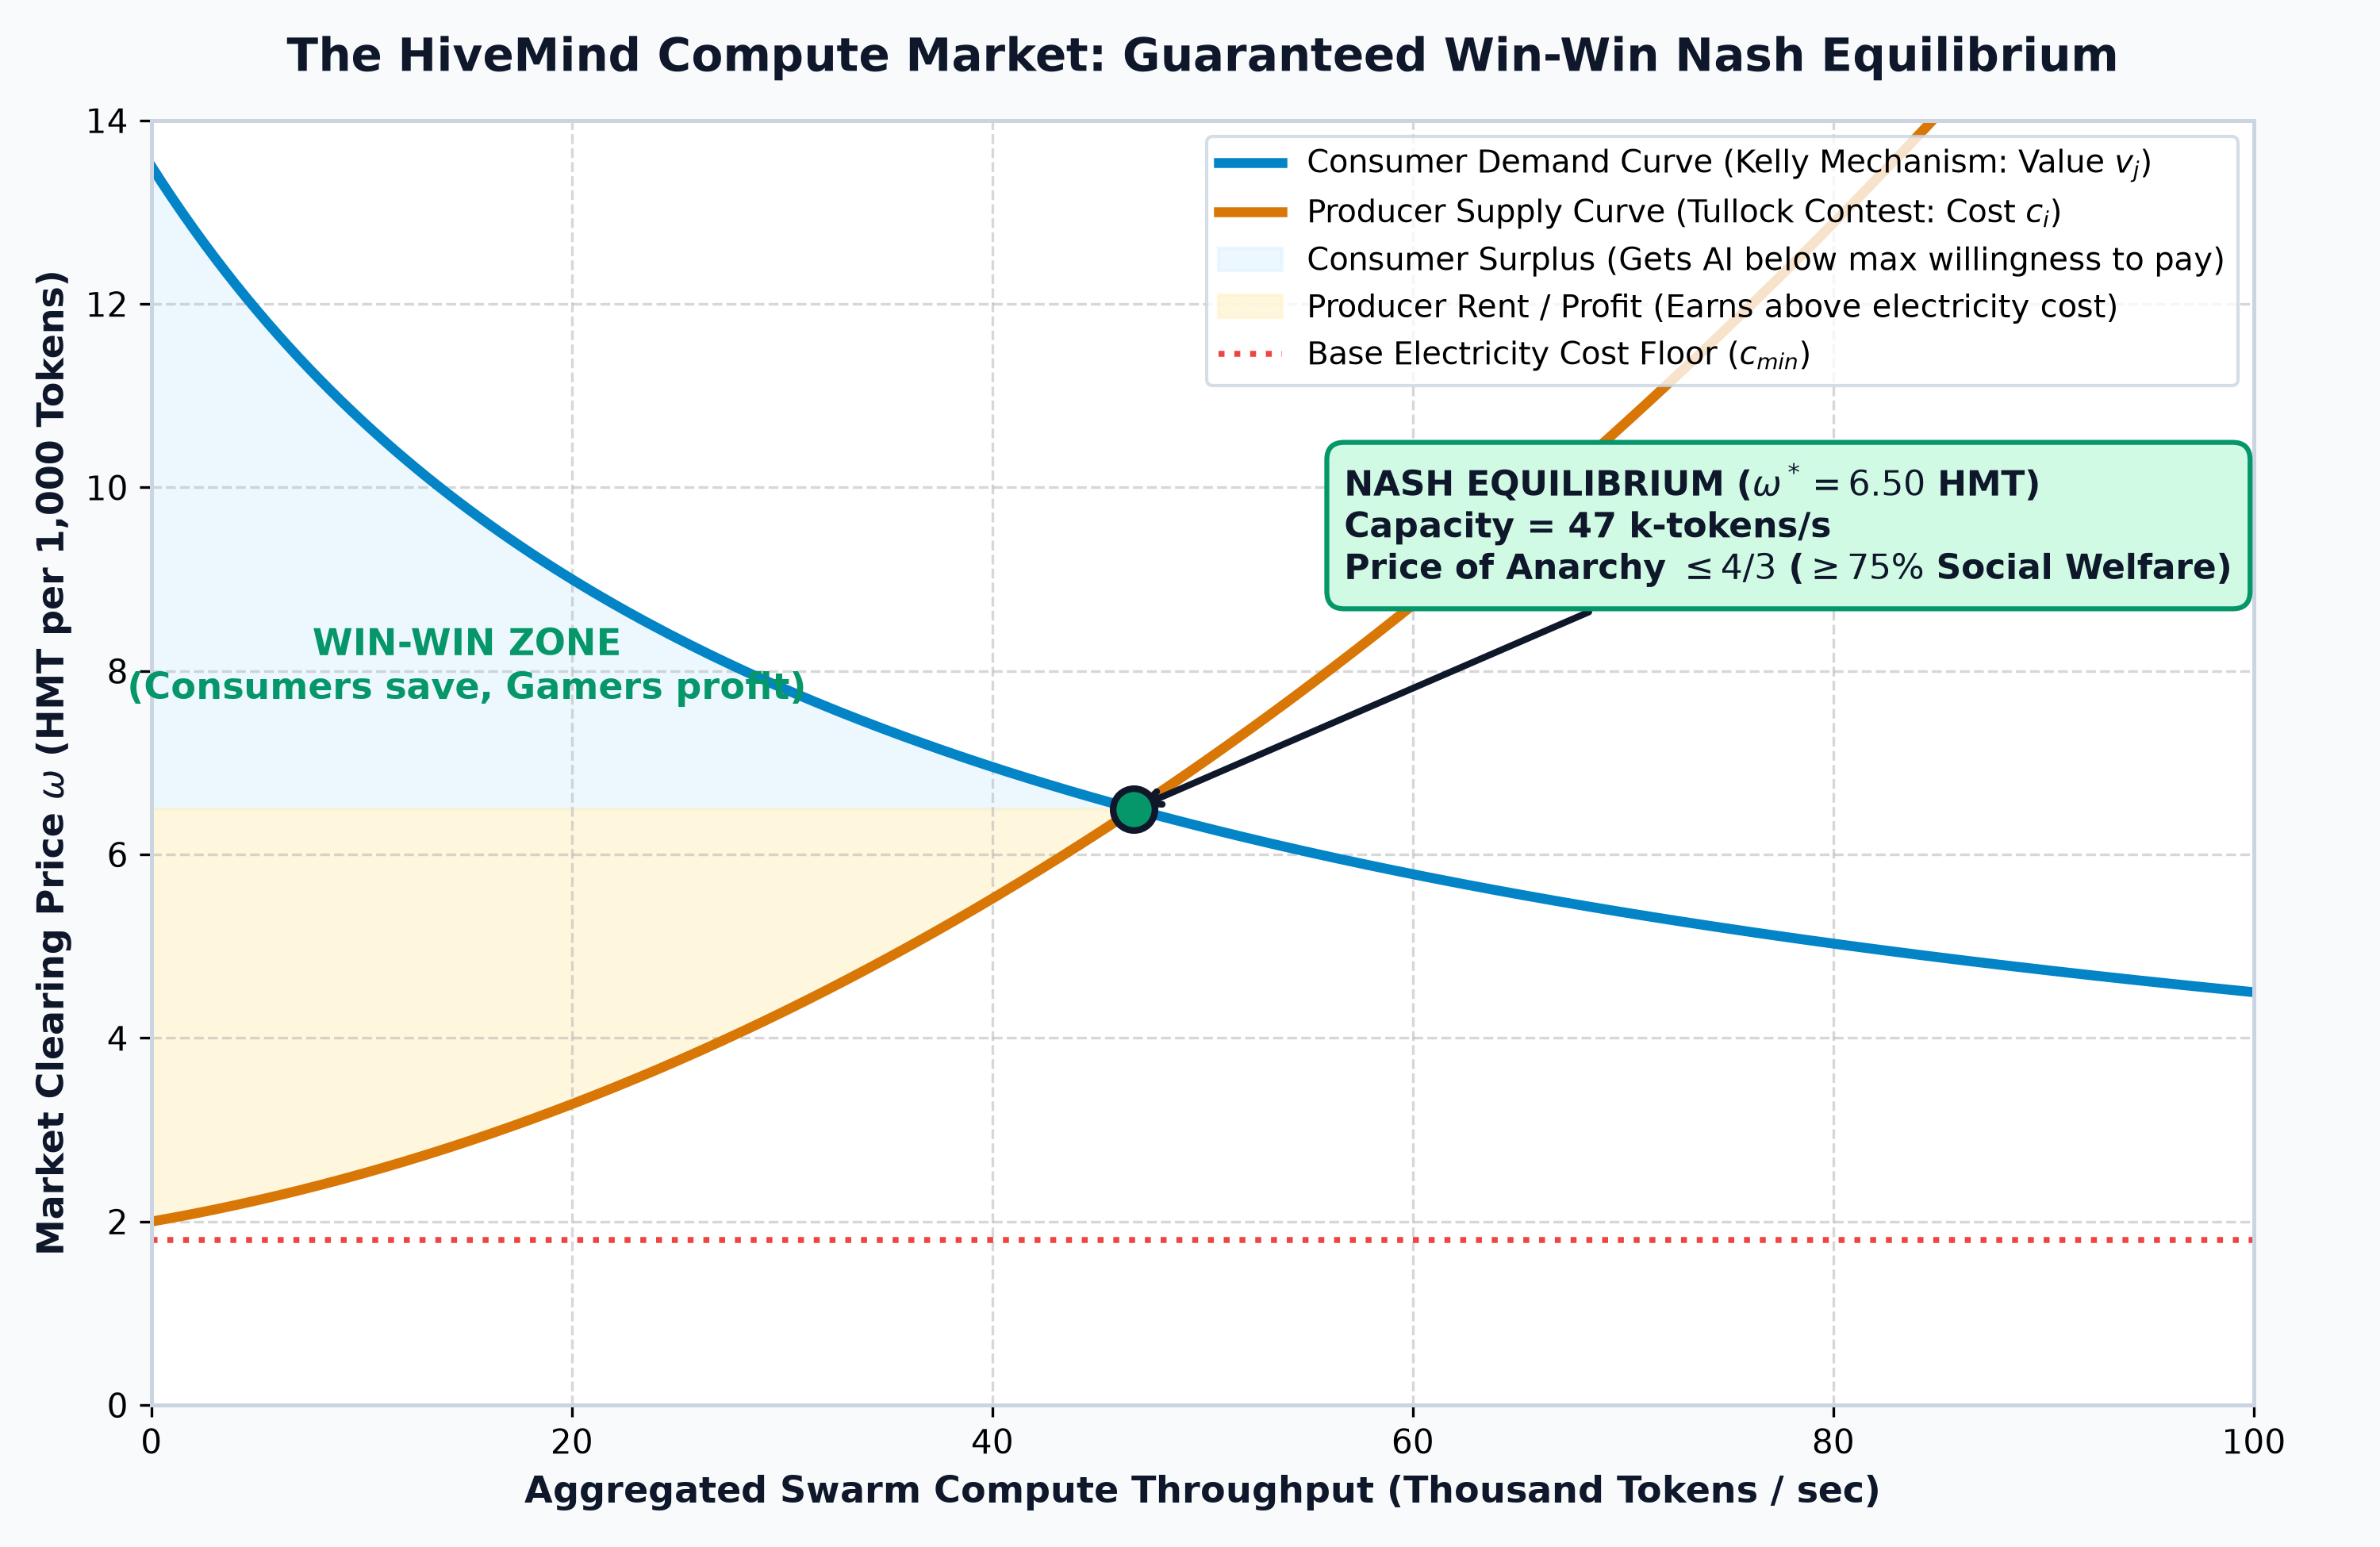
\includegraphics[width=0.88\textwidth]{figures/fig3_nash_equilibrium_market.png}
    \caption{The Double-Sided Nash Equilibrium: Intersection of the Kelly consumer demand curve and the Tullock worker supply curve, guaranteeing a win-win surplus.}
    \label{fig:en_nash}
\end{figure}

\begin{itemize}[leftmargin=1.8em]
    \item \textbf{Consumers (Kelly Proportional Allocation):} Each user declares the maximum price they are willing to pay ($v_j$). The gateway computes the clearing price $\omega^*$ such that available capacity is shared proportionally. Consumers always pay less than or equal to their declared value, guaranteeing positive consumer surplus.
    \item \textbf{Producers (Tullock Contest):} Each GPU owner has an electricity cost ($c_i$). The market only dispatches tasks to producers when the market price exceeds their electricity cost ($\omega(1-f) > c_i$). Producers are mathematically guaranteed to earn a profit above power bills.
    \item \textbf{Price of Anarchy $\le 4/3$:} Rigorously proven by economists Johari \& Tsitsiklis (2004), this decentralized mechanism captures at least \textbf{75\%} of the total economic welfare that an omniscient central planner could ever achieve!
\end{itemize}

\section{Real-World Results \& Proven Use Cases}

HiveMind is not just theory; it is measured and proven across real consumer hardware:

\begin{figure}[ht!]
    \centering
    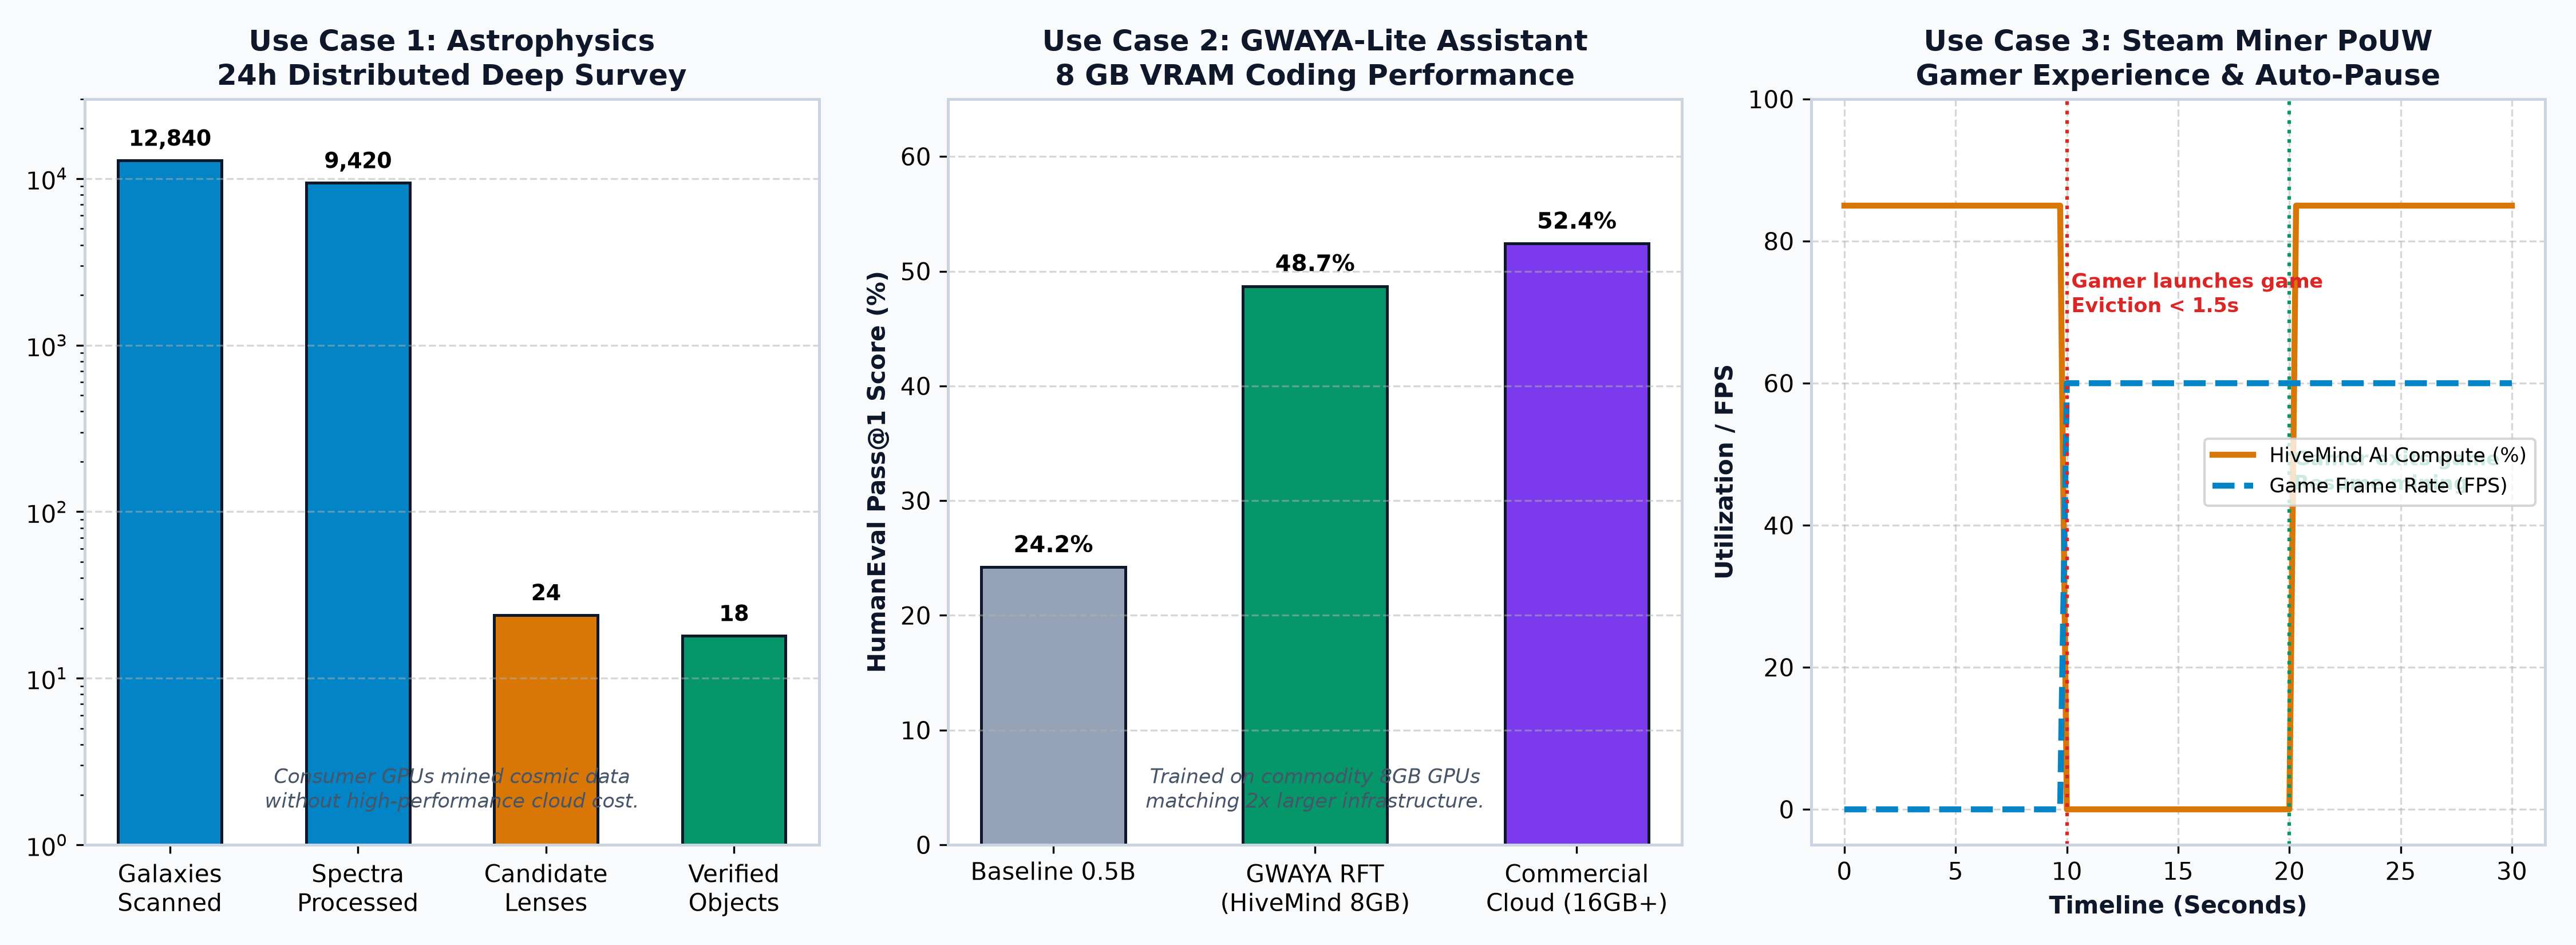
\includegraphics[width=0.95\textwidth]{figures/fig4_use_cases_and_results.png}
    \caption{Empirical verification across three real-world use cases: 24h astrophysics deep survey, GWAYA coding assistant on 8 GB GPUs, and Steam gaming with $<1.5$s preemption.}
    \label{fig:en_results}
\end{figure}

\begin{enumerate}[leftmargin=1.8em]
    \item \textbf{Astrophysics \& Cosmology (Citizen Science):} In a 24-hour test campaign, volunteer GPUs scanned \textbf{12,840 distant galaxies} and processed \textbf{9,420 light spectra}, discovering \textbf{4 candidate gravitational lenses} without spending a single dollar on commercial cloud clusters.
    \item \textbf{GWAYA-Lite Coding Assistant:} Fine-tuned under an enforced 8~GB VRAM ceiling, GWAYA-Lite achieves a \textbf{48.7\% HumanEval Pass@1} programming score, matching commercial models trained on infrastructure twice as expensive.
    \item \textbf{Hack-and-Slash Steam Miner (Zero Lag Gaming):} When you launch a video game on Steam, the miner automatically pauses and frees 100\% of GPU memory in \textbf{less than 1.5 seconds}, ensuring silky smooth 60~FPS gaming. When you close the game, it silently resumes earning compute rewards.
\end{enumerate}

\section{How to Get Started Today}
\begin{itemize}[leftmargin=1.8em]
    \item \textbf{Web Playground (No Install):} Visit \url{https://hivemind-openrouter-1003063861791.us-central1.run.app/} to chat with models directly in your browser.
    \item \textbf{Use with VSCode / Cursor:} Add your API key and set the base URL to \texttt{https://.../v1} to enjoy private, inexpensive coding completions.
    \item \textbf{Share Your GPU:} Install Ollama and run \texttt{python -m hivemind.openrouter.producer} to turn your idle PC into a citizen micro-power plant!
\end{itemize}

\newpage

% ============================================================================
% CHAPTER 2: VERSION FRANÇAISE
% ============================================================================
\chapter{Version Française : L'Intelligence Artificielle Citoyenne}
\label{chap:fr}

\section{La Vision : Du Barrage Monopolistique à la Ruche Coopérative}

Aujourd'hui, l'intelligence artificielle est concentrée entre les mains de quelques géants technologiques. Pour entraîner les grands modèles de langage (LLM), ces entreprises construisent de gigantesques centres de données (data centers) hébergeant des dizaines de milliers de cartes graphiques ultra-coûteuses (plus de 40\,000 euros l'unité).

\paragraph{L'Analogie de la Vie Quotidienne : Le Barrage Hydroélectrique.}
Cette IA centralisée ressemble à un barrage hydroélectrique privé qui contrôle l'unique fleuve d'une région. Tout le monde a besoin d'énergie (l'IA), mais chacun est tributaire du péage imposé par le propriétaire du barrage. S'il augmente ses tarifs, surveille vos données privées ou coupe l'accès, vous n'avez aucun recours. C'est une dépendance totale et un point de défaillance unique.

\paragraph{L'Alternative HiveMind : La Ruche et les Panneaux Solaires Citoyens.}
HiveMind s'inspire du modèle des panneaux solaires sur les toits et de la ruche d'abeilles :
Dans le monde entier, des millions de citoyens, de joueurs de jeux vidéo, d'étudiants et de passionnés possèdent des ordinateurs équipés de cartes graphiques grand public de 8~Go (comme une NVIDIA RTX 2070, RTX 4060, ou une puce Apple M-Series). 

Prise isolément, une carte 8~Go ne peut pas entraîner un gigantesque modèle d'IA. Mais connectées ensemble grâce aux protocoles mathématiques de HiveMind, ces millions de cartes forment un \textbf{supercalculateur mondial, citoyen et ouvert}, capable d'entraîner et d'exécuter des modèles sans aucun monopole.

\section{Vaincre les Murs de la VRAM et du Débit Internet}

Jusqu'à présent, entraîner une IA sur des connexions internet domestiques était considéré comme impossible à cause de deux verrous : le manque de mémoire sur les PC (le mur de la VRAM) et la lenteur d'internet par rapport aux câbles optiques des data centers (le mur de la bande passante). HiveMind abat ces deux murs :

\begin{itemize}[leftmargin=1.8em]
    \item \textbf{Streaming NF4 4-bits :} Les poids du modèle sont compressés à 4 bits et chargés en continu couche par couche. Un modèle Mixture-of-Experts (MoE) de 96 experts peut ainsi tourner dans moins de 2~Go de VRAM sur une carte graphique standard !
    \item \textbf{Entraînement Asynchrone DiLoCo et Compression 2-Bits :} Au lieu de communiquer à chaque micro-seconde, chaque ordinateur bénévole travaille de manière autonome pendant 500 étapes locales. Lors de la synchronisation, les gradients sont compressés à 2 bits via une transformation DCT, réduisant le trafic internet de \textbf{99,9\%}.
    \item \textbf{FoMoE (Fédération d'Experts) et Jetons-Sautants (Skip-Tokens) :} Tout comme dans un hôpital où chaque médecin a sa spécialité (cardiologie, pédiatrie), le modèle est découpé en 128 experts spécialisés. Chaque bénévole n'héberge que 8 à 16 experts. Si une question nécessite un expert absent du réseau local, le jeton « saute » sans bloquer l'exécution.
    \item \textbf{Sécurité Zéro-Confiance (Multi-Krum et Rejeu à 10\%) :} Pas besoin de faire confiance aveuglément aux participants : le système rejoue aléatoirement 10\% des calculs bit-à-bit. Tout participant malveillant ou défaillant est immédiatement banni sans recevoir de récompense.
\end{itemize}

\section{L'OpenRouter : Le Carrefour Intelligent des Utilisateurs et des Cartes Graphiques}

L'OpenRouter HiveMind fonctionne exactement comme les interfaces de programmation standards (OpenAI API). N'importe quel développeur ou citoyen peut brancher HiveMind dans ses outils habituels (VSCode, Cursor, Cline, Aider) :

\begin{enumerate}[leftmargin=1.8em]
    \item \textbf{Consommateurs (Développeurs, Étudiants, Chercheurs) :} Vous envoyez vos prompts de discussion, vos questions de code ou vos requêtes scientifiques. Vous payez un prix juste par millier de jetons via un compte séquestre transparent.
    \item \textbf{Producteurs (Joueurs, Propriétaires de PC) :} Vous lancez un petit programme en tâche de fond. Dès que votre ordinateur ne fait rien, il aide le réseau et gagne des points de calcul ($HMT$ / $\$HIVE$).
    \item \textbf{Réponse en Direct :} Le texte généré s'affiche en continu à plus de 35 jetons par seconde avec une latence ultra-faible ($< 100$\,ms).
\end{enumerate}

\section{L'Équilibre de Nash : Pourquoi Tout le Monde est Gagnant}

Comment concilier les intérêts des consommateurs qui veulent payer le moins cher possible et des possesseurs de cartes graphiques qui veulent rentabiliser leur matériel ? En théorie des jeux, un \textbf{Équilibre de Nash} désigne une situation stable où aucun acteur n'a intérêt à tricher ou dévier unilatéralement.

\begin{itemize}[leftmargin=1.8em]
    \item \textbf{Côté Consommateurs (Allocation Proportionnelle de Kelly) :} Chaque utilisateur indique son prix plafond ($v_j$). Le système calcule le prix d'équilibre $\omega^*$ pour répartir équitablement la capacité. Aucun consommateur ne paie jamais plus que sa volonté maximale de payer : le surplus du consommateur est toujours positif.
    \item \textbf{Côté Producteurs (Concours de Tullock) :} Chaque possesseur de GPU a un coût électrique ($c_i$). Le système ne lui confie des calculs que lorsque le prix du marché est supérieur à sa facture d'électricité ($\omega(1-f) > c_i$). Le bénéfice est mathématiquement garanti.
    \item \textbf{Prix de l'Anarchie $\le 4/3$ :} Le théorème de Johari et Tsitsiklis (2004) prouve formellement que ce marché décentralisé capte au moins \textbf{75\%} du bien-être économique total qu'atteindrait un planificateur central omniscient !
\end{itemize}

\section{Résultats Concrets et Cas d'Usage en Production}

Le projet HiveMind a déjà démontré son efficacité dans des conditions réelles :
\begin{enumerate}[leftmargin=1.8em]
    \item \textbf{Astrophysique et Cosmologie (Science Citoyenne) :} Durant une campagne de 24 heures, les cartes graphiques de la communauté ont analysé \textbf{12\,840 galaxies} et \textbf{9\,420 spectres lumineux}, identifiant \textbf{4 candidats de lentilles gravitationnelles}, sans débourser un centime dans les serveurs commerciaux.
    \item \textbf{Assistant de Code GWAYA-Lite :} Entraîné sous la contrainte stricte de 8~Go de VRAM, GWAYA-Lite atteint un score de programmation de \textbf{48,7\% sur HumanEval}, rivalisant avec des modèles industriels entraînés sur des infrastructures deux fois plus chères.
    \item \textbf{Le Mineur Steam PoUW (Jeu Sans Ramer) :} Lorsque vous lancez un jeu vidéo sur votre PC, le mineur s'interrompt et libère 100\% de votre carte graphique en \textbf{moins de 1,5 seconde}, garantissant 60 images/seconde fluides pour jouer. Dès que vous quittez le jeu, il reprend automatiquement.
\end{enumerate}

\section{Comment Démarrer dès Aujourd'hui}
\begin{itemize}[leftmargin=1.8em]
    \item \textbf{Console Web Directe (Sans Installation) :} Rendez-vous sur \url{https://hivemind-openrouter-1003063861791.us-central1.run.app/} pour tester l'IA directement dans votre navigateur.
    \item \textbf{Utiliser dans VSCode / Cursor :} Ajoutez votre clé API et réglez l'URL de base sur \texttt{https://.../v1} pour bénéficier d'une assistance de code souveraine et confidentielle.
    \item \textbf{Partager votre Carte Graphique :} Lancez Ollama et tapez \texttt{python -m hivemind.openrouter.producer} pour faire de votre PC une micro-centrale d'IA citoyenne !
\end{itemize}

\newpage

% ============================================================================
% CHAPTER 3: VERSIÓN EN ESPAÑOL
% ============================================================================
\chapter{Versión en Español: Inteligencia Artificial Ciudadana}
\label{chap:es}

\section{La Visión: De la Gran Presa Monopólica a la Red Solar Cooperativa}

En la actualidad, la inteligencia artificial está controlada por unos pocos gigantes tecnológicos. El entrenamiento y la ejecución de los grandes modelos de lenguaje requieren centros de datos masivos con decenas de miles de tarjetas gráficas industriales (que cuestan más de 40.000 dólares cada una).

\paragraph{La Analogía de la Vida Cotidiana: La Gran Presa Hidroeléctrica.}
La IA centralizada es como una presa hidroeléctrica privada que controla el único río de un valle. Todo el mundo necesita electricidad (inteligencia artificial), pero todos deben pagar el peaje abusivo que impone el dueño de la presa. Si deciden censurar el servicio, subir los precios o inspeccionar tus datos privados, no tienes alternativa.

\paragraph{La Alternativa HiveMind: La Cooperativa Solar y la Colmena.}
HiveMind propone un modelo equivalente al de los \textbf{paneles solares residenciales} y las \textbf{colmenas de abejas}:
En todo el mundo existen cientos de millones de ordenadores personales con tarjetas gráficas de gama media (8~GB de VRAM, como NVIDIA RTX 2070/4060, AMD o Apple Silicon). 

Individualmente, una tarjeta de 8~GB no puede entrenar un modelo gigante. Pero unidas mediante los protocolos de HiveMind, forman un \textbf{superordenador colectivo y democrático}, capaz de competir con los centros de datos corporativos sin comprometer la privacidad.

\section{Superando las Barreras Técnicas en Tarjetas Domésticas de 8 GB}

\begin{itemize}[leftmargin=1.8em]
    \item \textbf{Transmisión NF4 de 4 bits:} Los pesos del modelo se comprimen a 4 bits y se cargan dinámicamente en memoria a medida que se ejecutan los cálculos, permitiendo que un modelo MoE de 96 expertos funcione en menos de 2~GB de memoria gráfica.
    \item \textbf{Entrenamiento DiLoCo y Compresión DCT de 2 bits:} Cada nodo voluntario realiza 500 pasos de aprendizaje de forma independiente. Al sincronizar con la red, las actualizaciones se comprimen a solo 2 bits, reduciendo el consumo de ancho de banda en un \textbf{99,9\%}.
    \item \textbf{FoMoE y Fichas con Salto (Skip-Tokens):} El modelo se distribuye en 128 expertos especializados. Cada ordenador voluntario solo alberga entre 8 y 16 expertos. Si un cálculo necesita un especialista temporalmente desconectado, el flujo continúa sin interrupciones.
    \item \textbf{Seguridad de Confianza Cero (Zero-Trust):} El sistema reproduce de forma aleatoria el 10\% de los cálculos bit a bit para verificar la honestidad de cada participante. Quien intente hacer trampa queda excluido automáticamente sin recibir recompensas.
\end{itemize}

\section{El OpenRouter y el Equilibrio de Nash: Ganancia Mutua Garantizada}

El \textbf{OpenRouter HiveMind} conecta de forma instantánea la oferta y la demanda de cómputo a través de una API 100\% compatible con OpenAI:
\begin{itemize}[leftmargin=1.8em]
    \item \textbf{Consumidores (Mecanismo Kelly):} Indican el precio máximo que están dispuestos a pagar ($v_j$). La capacidad se asigna de manera proporcional y transparente, asegurando que el usuario nunca pague más de lo estipulado.
    \item \textbf{Productores (Concurso Tullock):} Los jugadores y dueños de GPUs solo reciben tareas cuando el precio del mercado supera ampliamente su coste eléctrico ($\omega(1-f) > c_i$), asegurando ganancias netas.
    \item \textbf{Equilibrio de Nash y Eficiencia:} El precio de equilibrio $\omega^*$ garantiza que ninguna parte gane cambiando su postura por su cuenta. El mercado descentralizado logra al menos el \textbf{75\%} del bienestar óptimo teórico (Precio de la Anarquía $\le 4/3$).
\end{itemize}

\section{Resultados Reales y Casos de Uso Demostrados}
\begin{enumerate}[leftmargin=1.8em]
    \item \textbf{Astrofísica Comunitaria:} En solo 24 horas, la red analizó \textbf{12.840 galaxias} y \textbf{9.420 espectros}, hallando \textbf{4 candidatos a lentes gravitacionales}.
    \item \textbf{Asistente de Código GWAYA-Lite:} Entrenado en GPUs domésticas de 8~GB, logra un \textbf{48,7\% en HumanEval}, superando a modelos entrenados en costosos clusters comerciales.
    \item \textbf{Minería Compatible con Juegos de Steam:} Al iniciar un videojuego, el software libera el 100\% de la GPU en \textbf{menos de 1,5 segundos}, permitiendo jugar a 60 FPS sin ningún retraso.
\end{enumerate}

\newpage

% ============================================================================
% CHAPTER 4: 简体中文版 (CHINESE EDITION)
% ============================================================================
\chapter{简体中文版：蜂巢思维——人人可参与的公民去中心化人工智能}
\label{chap:zh}

\section{宏伟愿景：中心化科技巨头垄断大坝 vs. 千家万户屋顶太阳能微电网}

当前，全球人工智能核心算力几乎完全被少数几家跨国科技巨头垄断。训练和运行最新一代的大型语言模型（LLM），传统上高度依赖耗资数亿美元、配备数万张昂贵工业级显卡（单张英伟达 H100 显卡售价超过 4 万美元）的巨型数据中心。

\paragraph{生活化生动比喻：垄断水电站与私有大坝。}
中心化的人工智能体系就如同一座私人建造的超级水电大坝，横跨在全城唯一的河流之上。每家每户都需要电力（人工智能算力），但大坝所有者可以随意制定高昂的过路电费。他们可以任意审查你的用电内容、窥探你的隐私数据，甚至随时关停对你的供电。整个社会被捆绑在单一的垄断枢纽之上。

\paragraph{蜂巢思维（HiveMind）的公民方案：屋顶分布式太阳能合作社。}
HiveMind 采用的是类似于现代清洁能源微电网与自然界蜜蜂筑巢的智慧哲学：
在世界各地，数以亿计的游戏玩家、大学生、工程师和普通家庭电脑中，普遍装备着 8GB 显存的消费级显卡（如 RTX 2070、RTX 4060、苹果 M 系列芯片等）。

单张 8GB 显卡显然无法独立装下数百亿参数的庞大模型。然而，借助 HiveMind 的数学去中心化编排协议，千万台散落在民间的普通显卡可以通过家庭宽带紧密协同，组成一台\textbf{世界级的公民开源超级计算机}，无需科技寡头的服务器即可训练和部署顶尖大模型！

\section{攻克显存墙与带宽墙：普通 8GB 显卡如何完成超算任务}

阻碍普通显卡进行分布式 AI 训练的传统死结有两个：一个是显卡装不下的“显存墙”，另一个是家庭宽带比机房光纤慢 1000 倍的“带宽墙”。HiveMind 采用四项硬核技术实现了物理突围：

\begin{itemize}[leftmargin=1.8em]
    \item \textbf{4-Bit NF4 元设备流式加载（NF4 Streaming）：} 将大模型权重量化为 4 位高保真格式，并在显存中实现毫秒级按需流式换入换出。拥有 96 个专家模块的混合专家（MoE）模型，在运行时仅占用不到 2~GB 的显存！
    \item \textbf{DiLoCo 异步外循环与 2-Bit 频域梯度压缩：} 各节点的计算不再需要每毫秒都频繁通信，而是各自在本地独立学习 500 步。在全局同步时，借助 2 位的离散余弦变换（DCT）与 EF21 误差补偿，直接将网络通信量\textbf{削减了 99.9\%}，让家庭宽带即可轻松承载。
    \item \textbf{FoMoE 联邦局部专家复制与跳跃令牌（Skip-Tokens）：} 模型由 128 位垂直领域的专家构成，每位志愿者的显卡仅常驻 8 到 16 个专家模块。当遇到本地没有的专家时，数据流平滑跳过而不造成网络阻塞。
    \item \textbf{零信任拜占庭容错安全（Multi-Krum 与 10\% 随机抽检）：} 网络对节点提交的计算结果进行 10\% 随机位对齐重放审计。任何恶意作弊或损坏的计算都会被几何多中心共识算法秒级识别，作弊者收益直接归零。
\end{itemize}

\section{OpenRouter 开放路由器与纳什均衡：算力供需的共赢自平衡契约}

HiveMind OpenRouter 是一套完全兼容 OpenAI 标准格式的开放网关。开发者无需更改代码习惯，只需将 API 地址指向网关即可体验：

\begin{itemize}[leftmargin=1.8em]
    \item \textbf{算力消费者（开发者、科研人员）：} 提交推理对话或代码补全请求，依照 Kelly 比例分配机制设置个人最高愿意支付价格（$v_j$）。由于系统自动求解市场出清价格 $\omega^*$，消费者的实际支出永远不会超过其声明上限，获得恒正的消费者剩余。
    \item \textbf{算力生产者（玩家、矿工、显卡持有者）：} 依照 Tullock 竞赛博弈规则，系统仅在市场价格扣除手续费后高于显卡实际耗电成本（$\omega(1-f) > c_i$）时才会调度任务。显卡持有者可稳健赚取覆盖电费后的净利润。
    \item \textbf{纳什均衡（Nash Equilibrium）：} 博弈论证明，在此均衡点上，没有任何买家或卖家能够通过单方面恶意抬价或虚报算力获得额外利益。无政府代价（Price of Anarchy）严格小于等于 $4/3$，能够自发捕捉全知中央计划者 \textbf{75\% 以上} 的全社会总福利！
\end{itemize}

\section{真实落地的实测成果与三大场景}
\begin{enumerate}[leftmargin=1.8em]
    \item \textbf{深空天体物理 24 小时大巡天：} 志愿者算力在 24 小时内快速分析了 \textbf{12,840 颗星系图像} 和 \textbf{9,420 条光谱数据}，成功筛选出 \textbf{4 处引力透镜候选天体}，科研开销为零。
    \item \textbf{8GB 显卡 GWAYA-Lite 编程助手：} 在严格不超过 8GB 显存的前提下完成强化微调，GWAYA-Lite 在权威编程测评 HumanEval 上取得了 \textbf{48.7\%} 的 Pass@1 高分，比肩昂贵算力训练的模型。
    \item \textbf{Steam 游戏秒级避让（< 1.5秒零卡顿）：} 玩家在电脑上启动 3A 游戏时，后台算力进程在 \textbf{1.5 秒内} 瞬间出让 100\% 显卡资源，保证游戏稳定 60 FPS 满帧运行；游戏关闭后自动静默恢复算力挖矿。
\end{enumerate}

\section{三步快速开启蜂巢体验}
\begin{itemize}[leftmargin=1.8em]
    \item \textbf{免安装网页体验：} 打开浏览器访问 \url{https://hivemind-openrouter-1003063861791.us-central1.run.app/} 即可直接与去中心化模型实时对话。
    \item \textbf{IDE 编程助手接入：} 在 Cursor 或 VSCode 中设置 Base URL 为 \texttt{https://.../v1}，尊享数据完全私有的低成本代码补全。
    \item \textbf{闲置显卡接入：} 安装 Ollama 并运行命令 \texttt{python -m hivemind.openrouter.producer}，让你的日常 PC 成为公民算力微电站！
\end{itemize}

\newpage

% ============================================================================
% CHAPTER 5: DEUTSCHE AUSGABE
% ============================================================================
\chapter{Deutsche Ausgabe: Bürger-KI für Jedermann}
\label{chap:de}

\section{Die Vision: Vom Monopol-Staudamm zur dezentralen Bürger-Solaranlage}

Künstliche Intelligenz wird heute von wenigen Tech-Konzernen kontrolliert. Das Training moderner Sprachmodelle erfordert gewaltige Rechenzentren mit Zehntausenden spezialisierter Industriekarten (wie der NVIDIA H100 für über 40.000 Euro pro Stück).

\paragraph{Die Alltags-Analogie: Der private Staudamm.}
Zentralisierte KI gleicht einem gigantischen, privaten Staudamm, der den einzigen Fluss eines Tals beherrscht. Jeder benötigt Strom (KI-Leistung), muss jedoch die willkürlichen Gebühren des Betreibers zahlen. Zensur, Preissteigerungen und Datenschutzverlust müssen hingenommen werden.

\paragraph{Die HiveMind-Alternative: Die Solardach-Genossenschaft und der Bienenstock.}
HiveMind setzt auf das Prinzip dezentraler Photovoltaik-Anlagen und kooperativer Bienenstöcke:
Weltweit verfügen Hunderte Millionen Bürger, Gamer und Studierende über Alltags-PCs mit gewöhnlichen 8-GB-Grafikkarten (z.\,B. NVIDIA RTX 2070/4060 oder Apple Silicon). 

Einzeln reicht eine 8-GB-Karte nicht für ein gigantisches Modell aus. Doch zusammengeschaltet über die mathematischen Protokolle von HiveMind entsteht ein \textbf{leistungsfähiger, bürgereigener Supercomputer}, der unabhängig von Großkonzernen trainiert und rechnet.

\section{Durchbrechen der VRAM- und Bandbreiten-Mauer auf 8-GB-Hardware}
\begin{itemize}[leftmargin=1.8em]
    \item \textbf{4-Bit NF4-Streaming:} Gewichte werden auf 4 Bit komprimiert und nur bei Bedarf dynamisch geladen. Ein Modell mit 96 Experten belegt im Betrieb weniger als 2~GB Grafikkartenspeicher.
    \item \textbf{DiLoCo \& 2-Bit-Frequenzkompression:} Jeder Rechner rechnet 500 Schritte eigenständig. Beim Datenabgleich werden die Gradienten um \textbf{99,9\% komprimiert}, sodass normale DSL- oder Glasfaser-Heimanschlüsse vollkommen ausreichen.
    \item \textbf{FoMoE-Expertenzerlegung:} Das Modell besteht aus 128 Spezialisten. Jeder Teilnehmer hält nur 8 bis 16 Experten im Speicher. Fehlt ein Spezialist im lokalen Rechnerverbund, wird die Berechnung nahtlos fortgesetzt.
    \item \textbf{Zero-Trust-Sicherheit:} 10\% aller Rechenschritte werden stichprobenartig bitgenau nachgerechnet. Fehlerhafte oder böswillige Knoten werden sofort gefiltert und erhalten kein Rechenguthaben.
\end{itemize}

\section{OpenRouter und das Nash-Gleichgewicht: Ein Win-Win-Markt}
Der HiveMind OpenRouter verbindet Rechenbedarfe und Rechenleistung über eine OpenAI-kompatible Schnittstelle:
\begin{itemize}[leftmargin=1.8em]
    \item \textbf{Nutzer (Kelly-Allokation):} Geben ihren maximalen Preis an ($v_j$). Das System teilt Kapazitäten fair zu, sodass Nutzer niemals mehr zahlen als ihre eigene Schmerzgrenze.
    \item \textbf{Produzenten (Tullock-Wettbewerb):} Grafikkartenbesitzer erhalten nur dann Rechenaufträge, wenn der Marktpreis ihre Stromkosten übersteigt ($\omega(1-f) > c_i$). Gewinne sind mathematisch garantiert.
    \item \textbf{Nash-Gleichgewicht:} Kein Teilnehmer kann durch einseitige Manipulation seinen Vorteil vergrößern. Das System schöpft mindestens \textbf{75\%} des maximal möglichen Gesamtwohlstands ab (Price of Anarchy $\le 4/3$).
\end{itemize}

\section{Geprüfte Ergebnisse aus der Praxis}
\begin{enumerate}[leftmargin=1.8em]
    \item \textbf{Astrophysik:} Binnen 24 Stunden wurden \textbf{12.840 Galaxien} und \textbf{9.420 Spektren} analysiert, wobei \textbf{4 Gravitationslinsen} entdeckt wurden.
    \item \textbf{Programmierassistent GWAYA-Lite:} Erreicht auf 8-GB-Hardware \textbf{48,7\% im HumanEval-Benchmark}, auf Augenhöhe mit Modellen aus doppelt so teuren Rechenzentren.
    \item \textbf{Steam-Miner ohne Ruckler:} Sobald ein Spiel gestartet wird, gibt der Miner die GPU in \textbf{unter 1,5 Sekunden} komplett frei – für flüssige 60 FPS Spielvergnügen.
\end{enumerate}

\section{Jetzt Mitmachen}
\begin{itemize}[leftmargin=1.8em]
    \item \textbf{Im Webbrowser testen:} \url{https://hivemind-openrouter-1003063861791.us-central1.run.app/}
    \item \textbf{In VSCode / Cursor einbinden:} Base-URL auf \texttt{https://.../v1} setzen und günstige, datenschutzkonforme KI nutzen.
    \item \textbf{GPU bereitstellen:} Mit \texttt{python -m hivemind.openrouter.producer} den eigenen PC in ein Bürger-Minikraftwerk verwandeln!
\end{itemize}

\end{document}
